\documentclass{beamer} 
\usepackage{amsmath,amsthm}
\usepackage{graphicx,microtype,parskip}
\usepackage{caption,subcaption,multirow}
\usepackage{attrib}

\frenchspacing

\usetheme{default}
\usecolortheme{whale}

\setbeamertemplate{navigation symbols}{}

\setbeamercolor{title}{fg=blue,bg=white}

\setbeamercolor{block title}{fg=white,bg=gray}
\setbeamercolor{block body}{fg=black,bg=lightgray}

\setbeamercolor{block title alerted}{fg=white,bg=darkgray}
\setbeamercolor{block body alerted}{fg=black,bg=lightgray}

%\AtBeginSection[]
%{
%  \begin{frame}
%    \tableofcontents[currentsection]
%  \end{frame}
%}


\begin{document}

\begin{frame}
  \tableofcontents
\end{frame}

\section{Talks, travel, grants}
\begin{frame}
  \frametitle{Talks}

  \begin{itemize}
    \item Evolution 2014: basic comparison between NA and European mammal survival 
    \item GSA 2014: current fully Bayesian model of brachiopod survival
      \begin{itemize}
        \item lots of positive feedback, ideas
      \end{itemize}
  \end{itemize}
\end{frame}

\begin{frame}
  \frametitle{Travel and grants}

  \begin{itemize}
    \item AMNH: tooth measures for all notoungulate specimens identified to species level
    \item DDIG: travel to Argentina; collaboration with Rick Madden
  \end{itemize}
\end{frame}


\section{Brachiopods}
\begin{frame}
  \frametitle{Survival model development}
\end{frame}

\section{Mammals}
\begin{frame}
  \frametitle{North American survival}
\end{frame}

\begin{frame}
  \frametitle{Model diagram}
  \begin{center}
    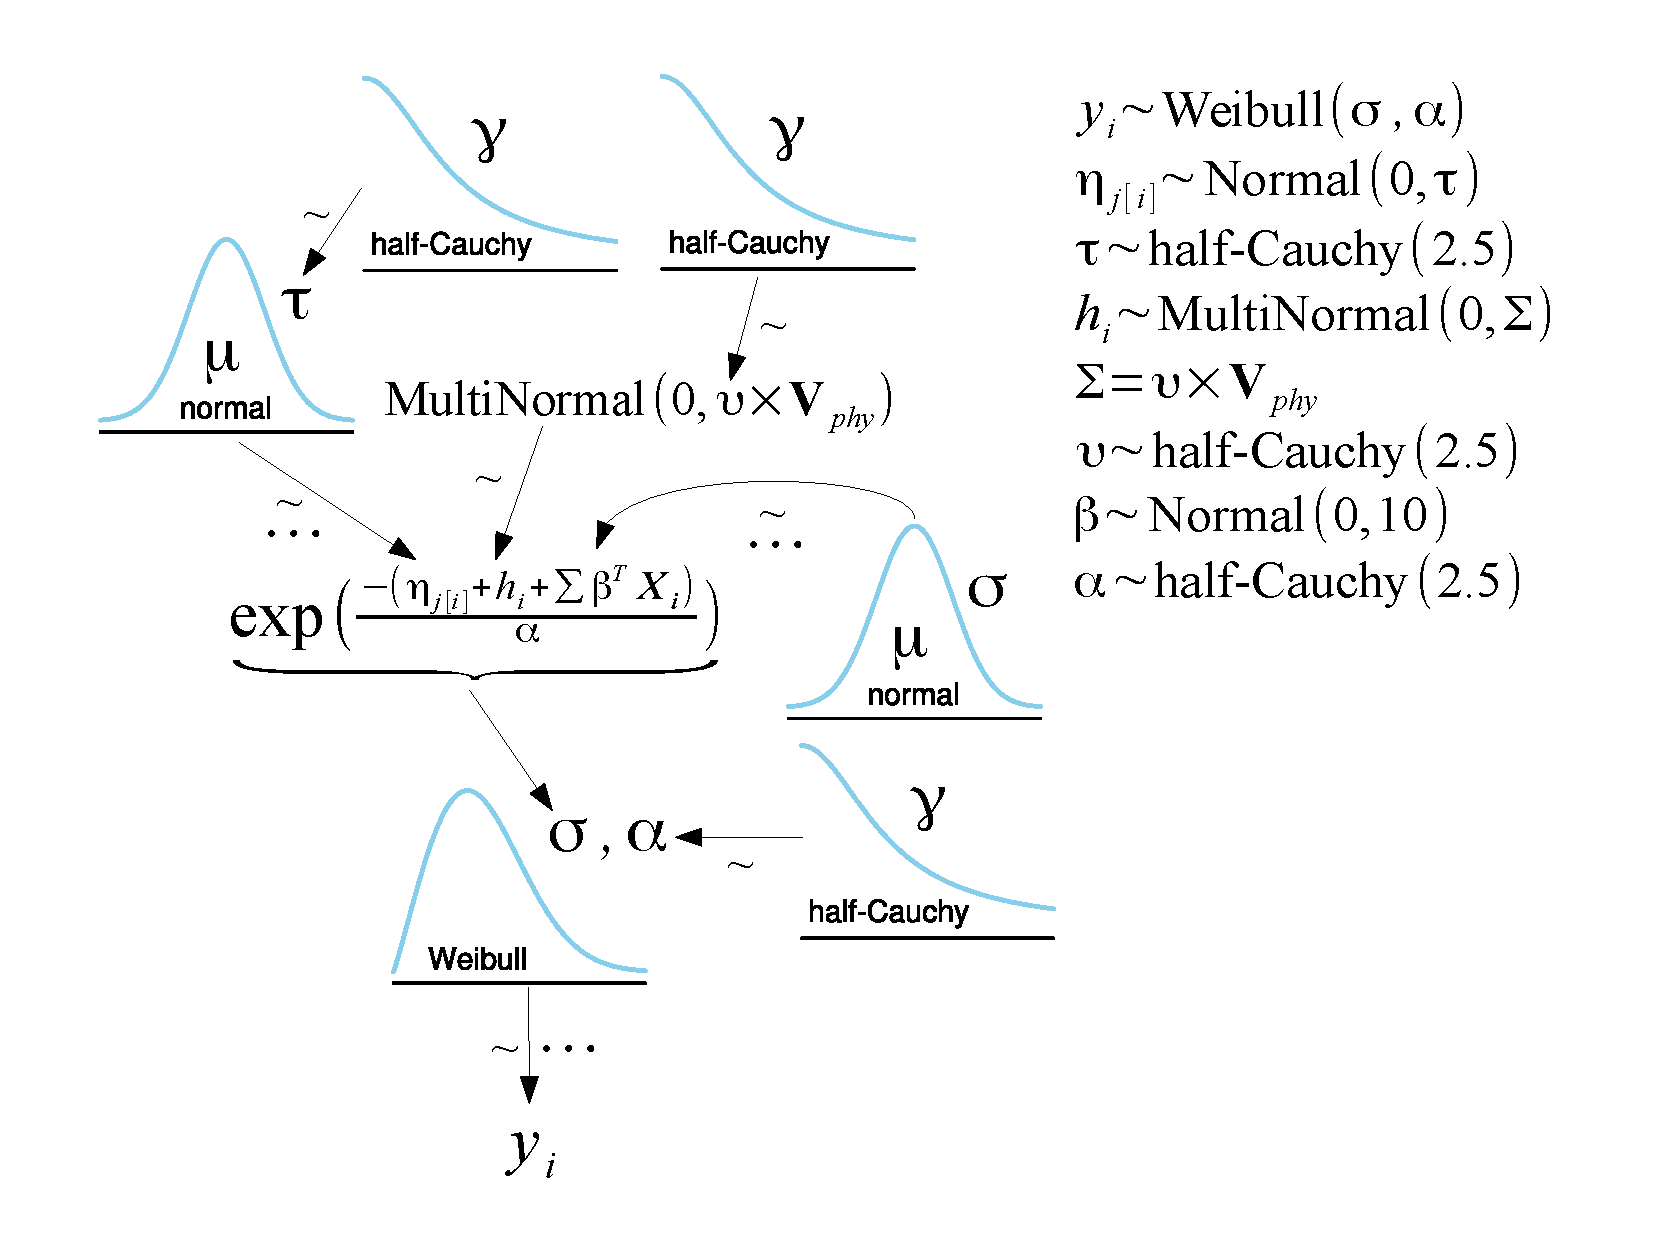
\includegraphics[height = 0.8\textheight, width = \textwidth,  keepaspectratio = true]{figure/mammal_survival_model}
  \end{center}
\end{frame}

\begin{frame}
  \frametitle{Posterior predictive checks: S(t)}
  \begin{center}
    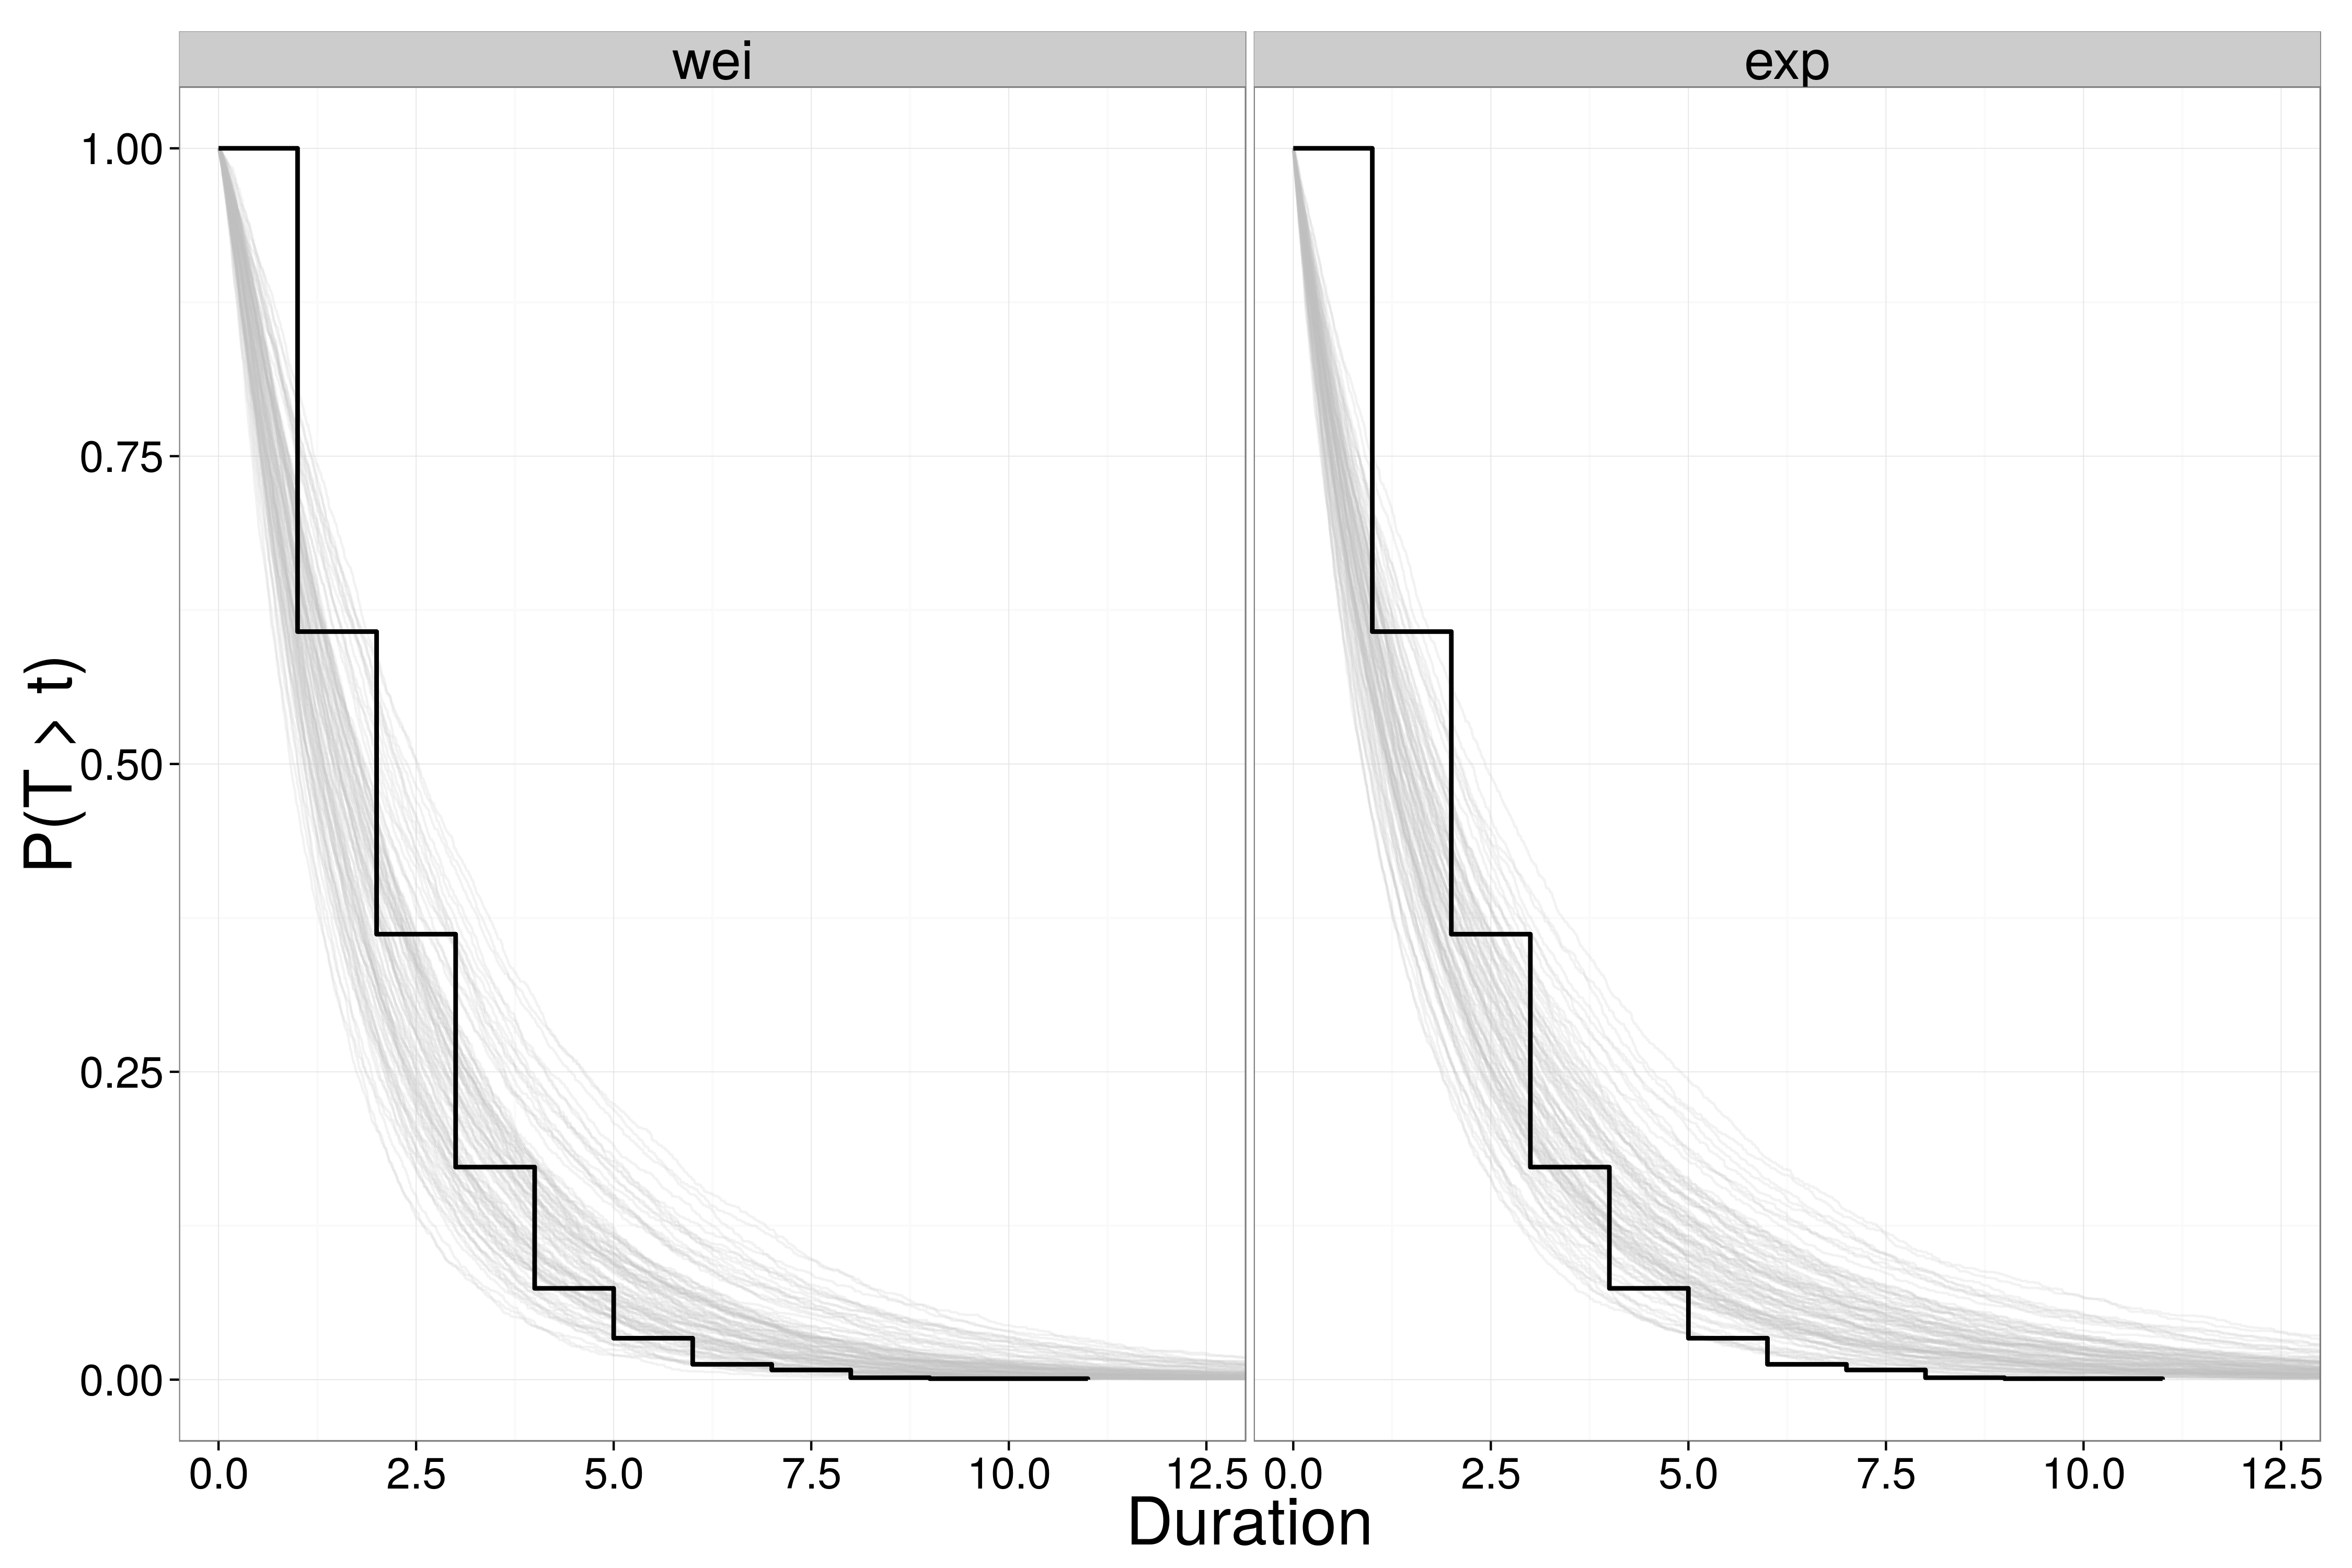
\includegraphics[height = 0.8\textheight, width = \textwidth,  keepaspectratio = true]{figure/survival_function}
  \end{center}
\end{frame}

\begin{frame}
  \frametitle{Posterior predictive checks: stnd. residuals}
  \begin{center}
    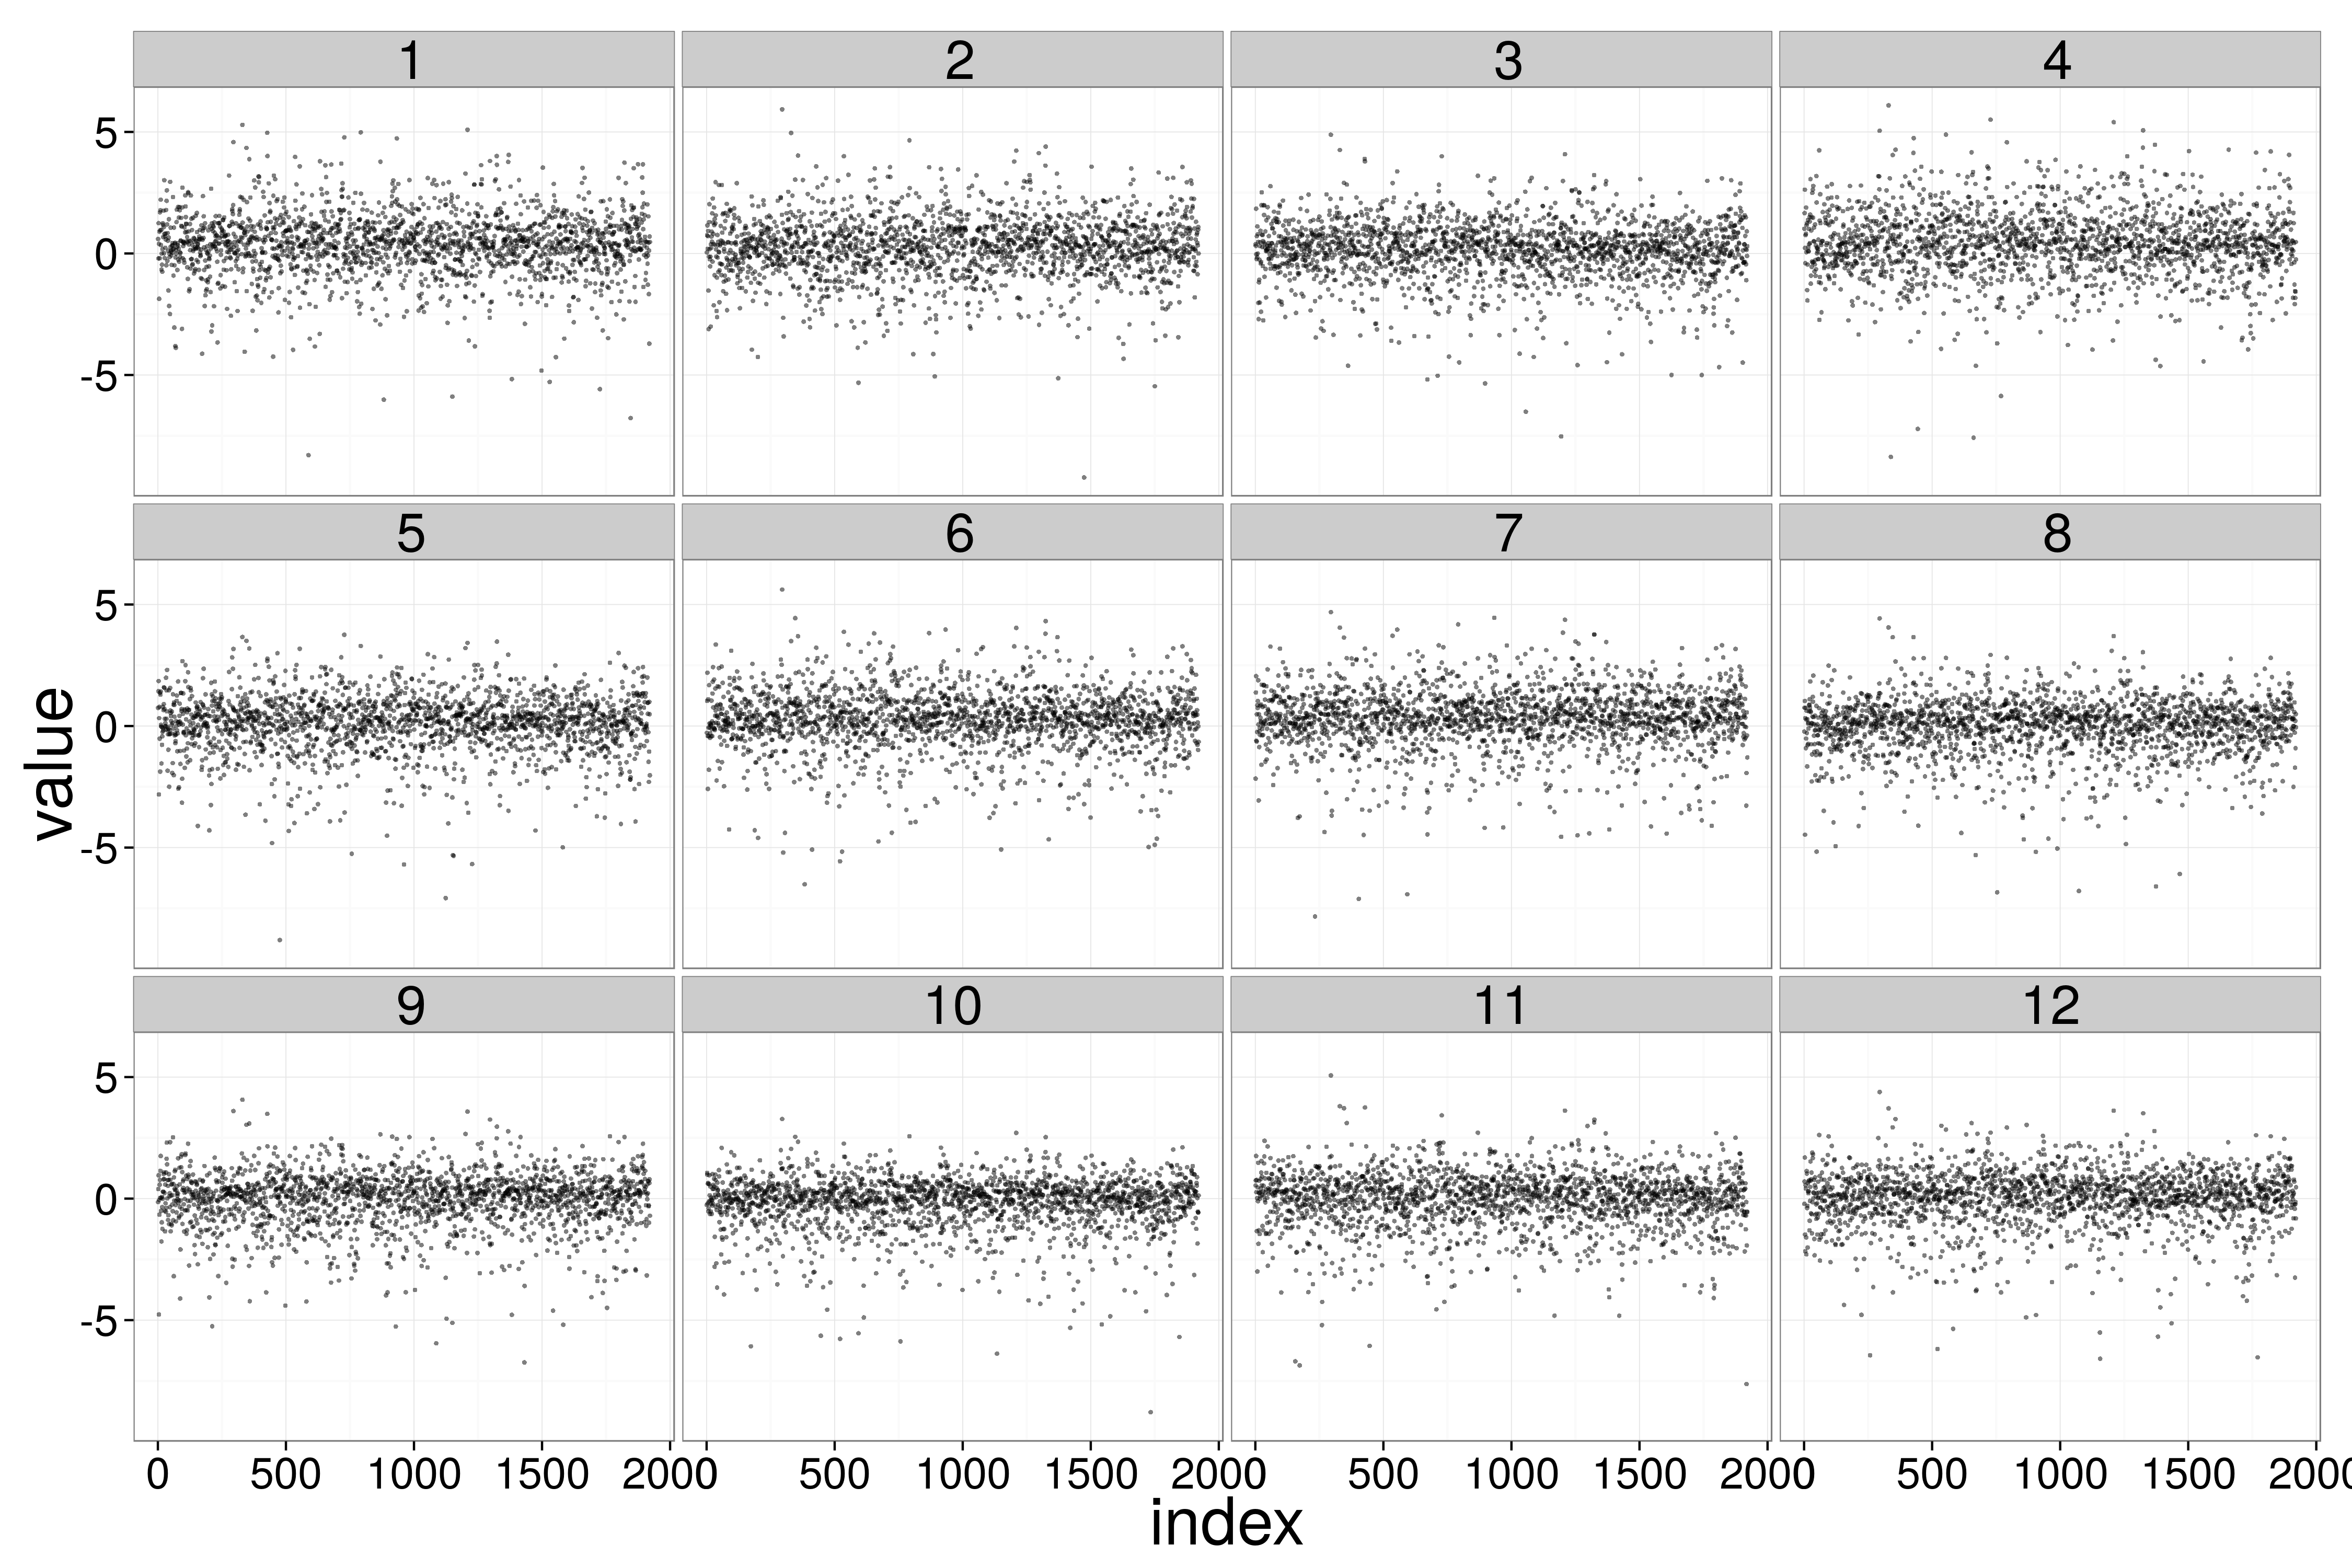
\includegraphics[height = 0.8\textheight, width = \textwidth,  keepaspectratio = true]{figure/residual_plot}
  \end{center}
\end{frame}

\begin{frame}
  \frametitle{Posterior predictive checks: residuals and mean}
  \begin{columns}
    \begin{column}{0.5\textwidth}
      \begin{center}
        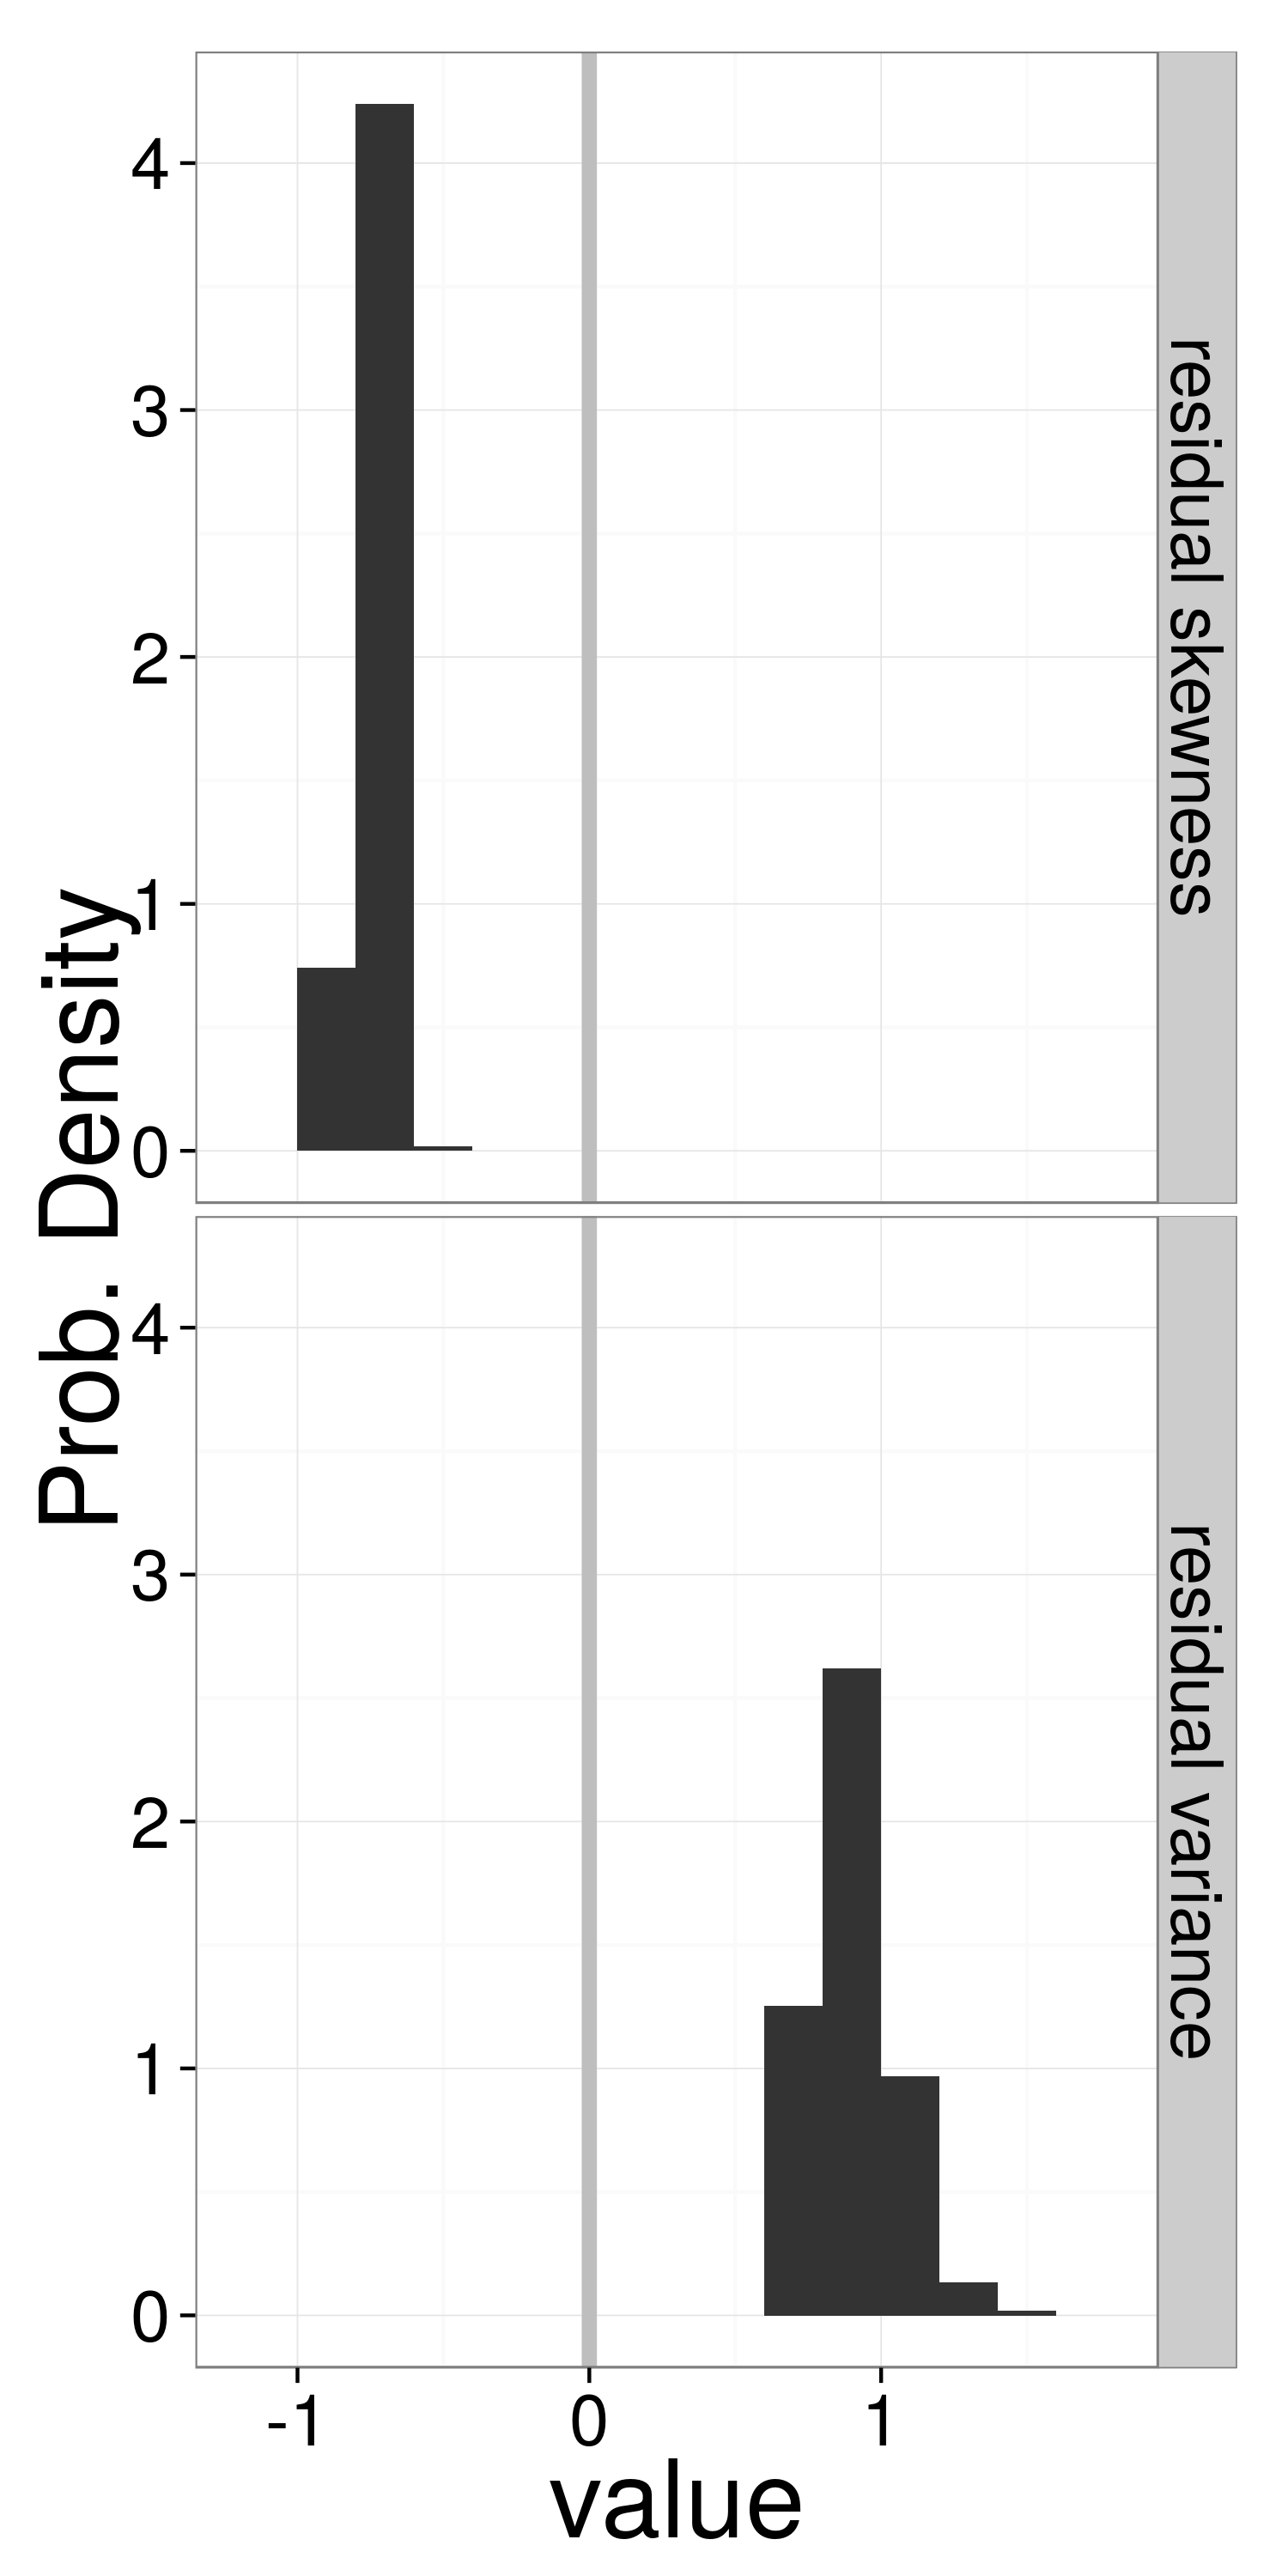
\includegraphics[height = 0.8\textheight, width = \textwidth,  keepaspectratio = true]{figure/res_sum_plot}
      \end{center}
    \end{column}
    \begin{column}{0.5\textwidth}
      \begin{center}
        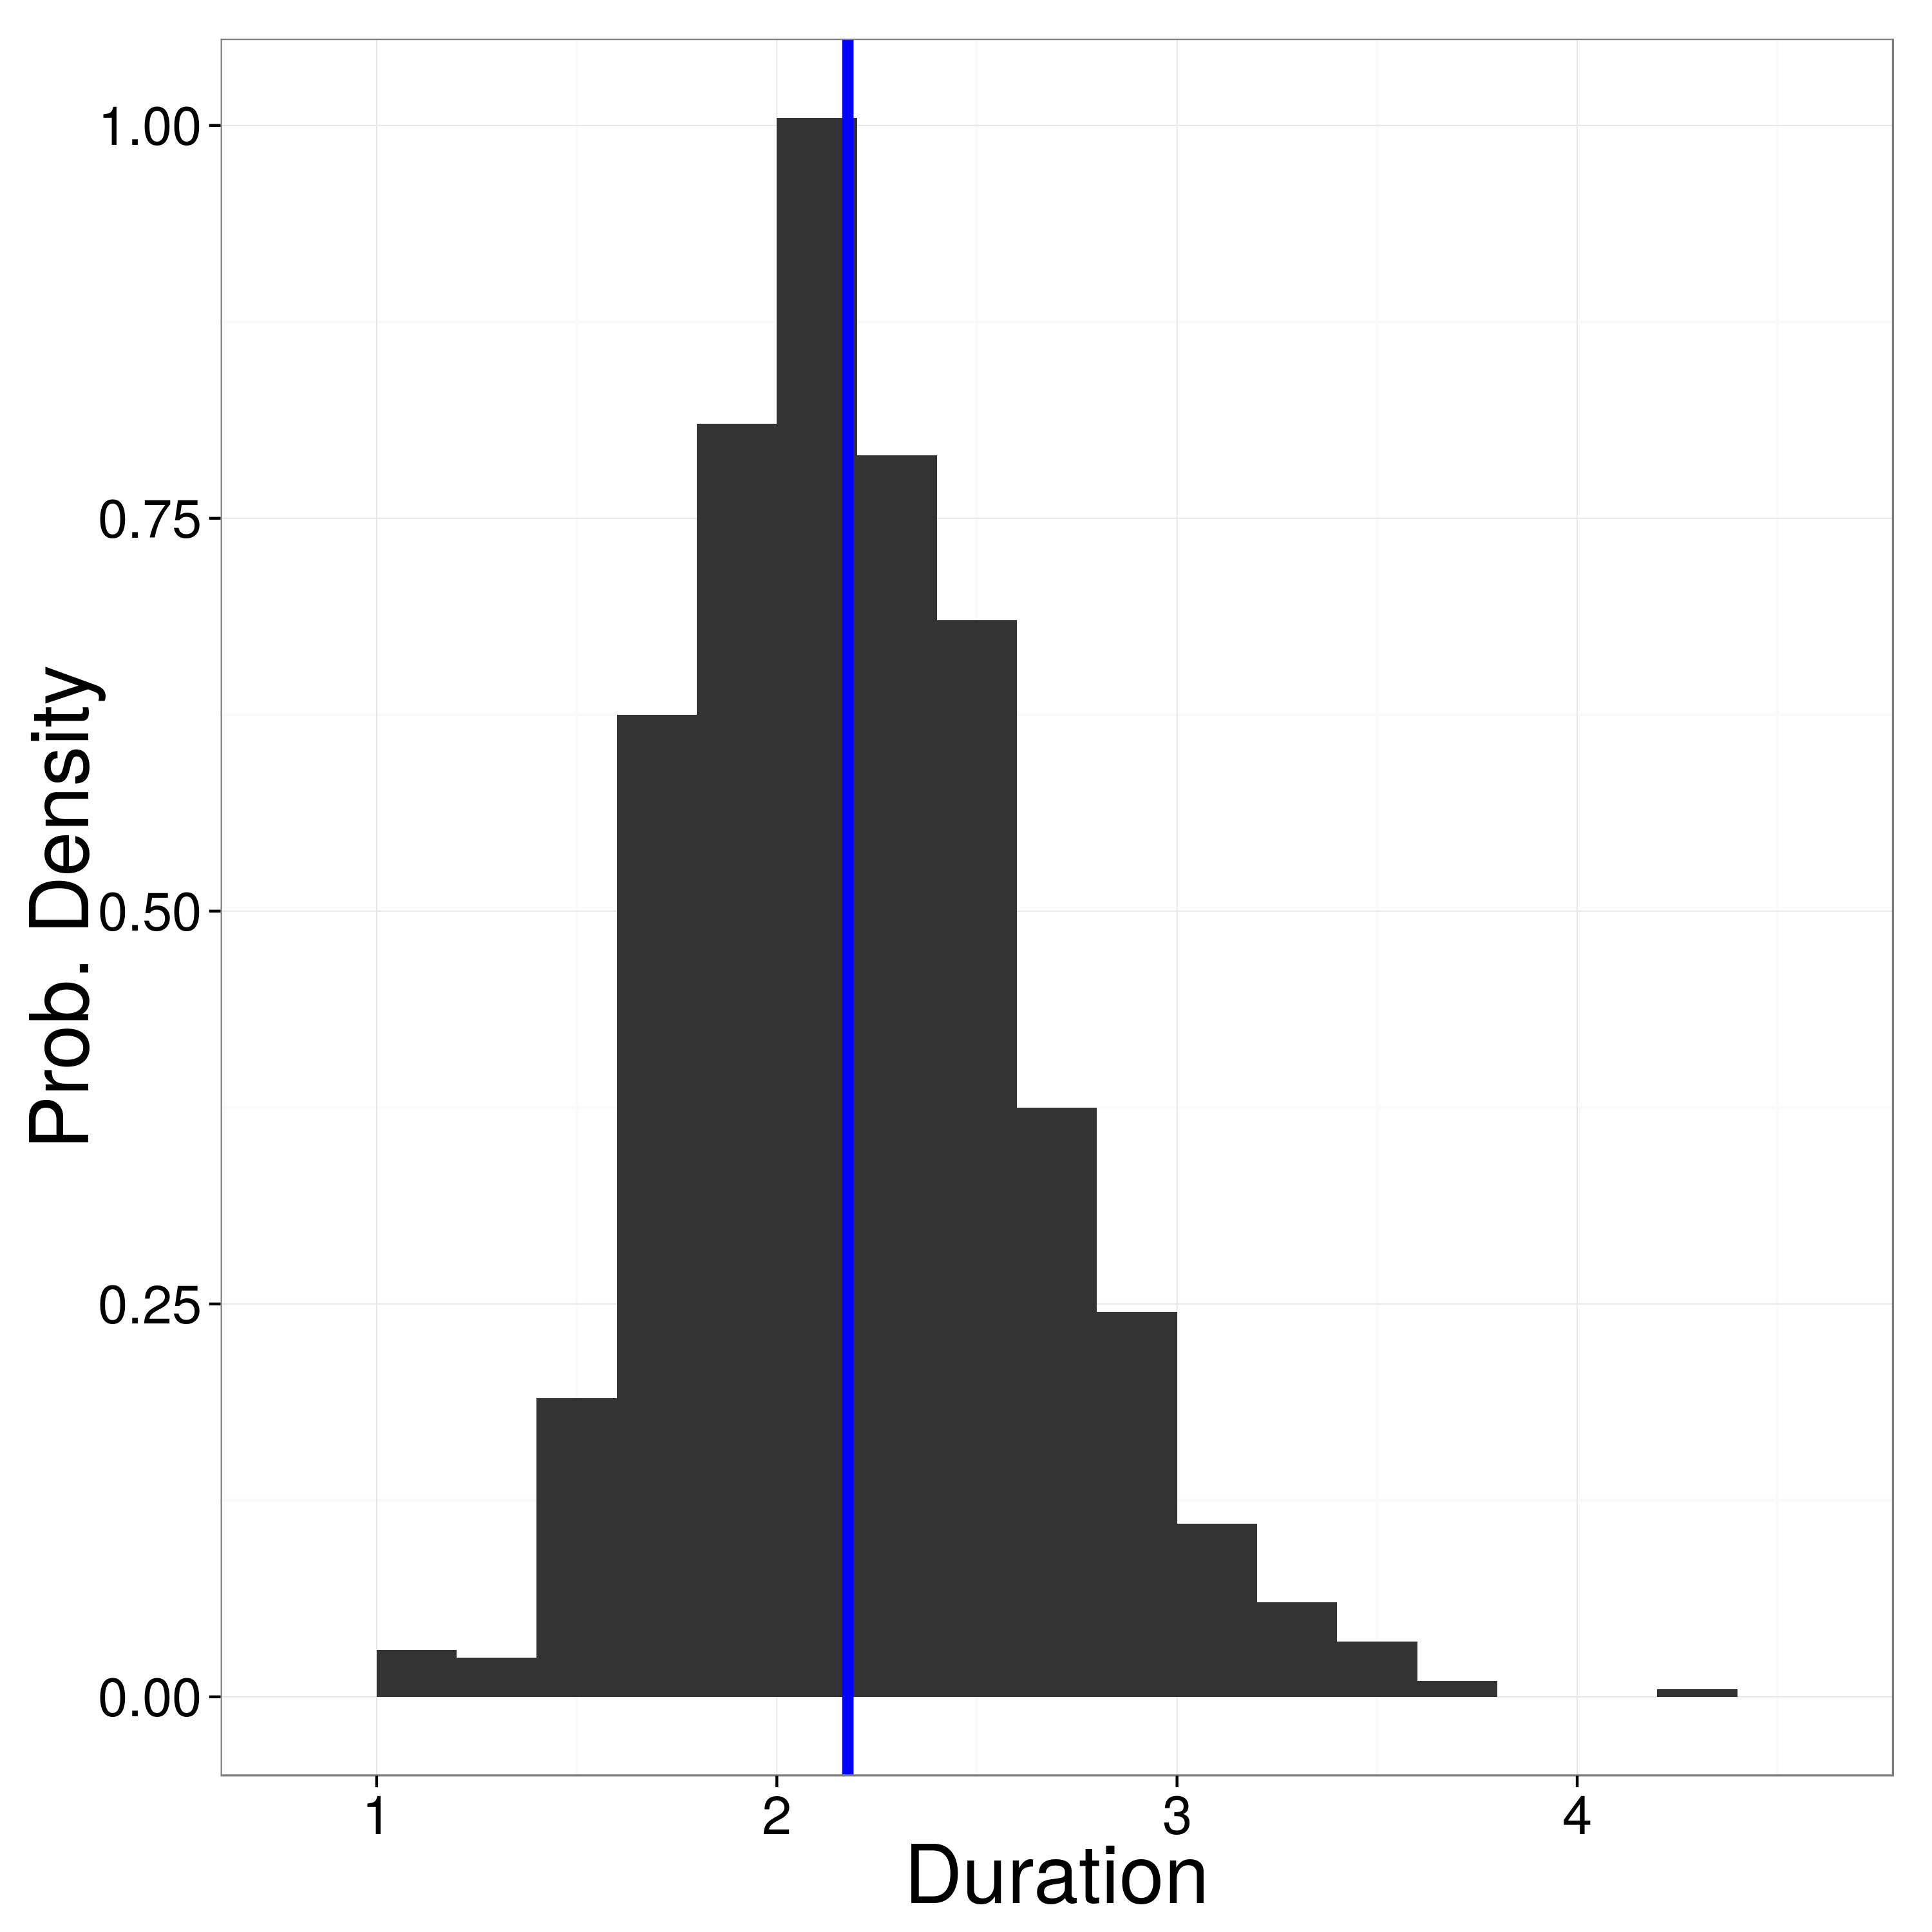
\includegraphics[height = 0.8\textheight, width = \textwidth,  keepaspectratio = true]{figure/mean_ppc}
      \end{center}
    \end{column}
  \end{columns}
\end{frame}

\begin{frame}
  \frametitle{Pairwise differences of \(\beta\), dietary category}
  \begin{center}
    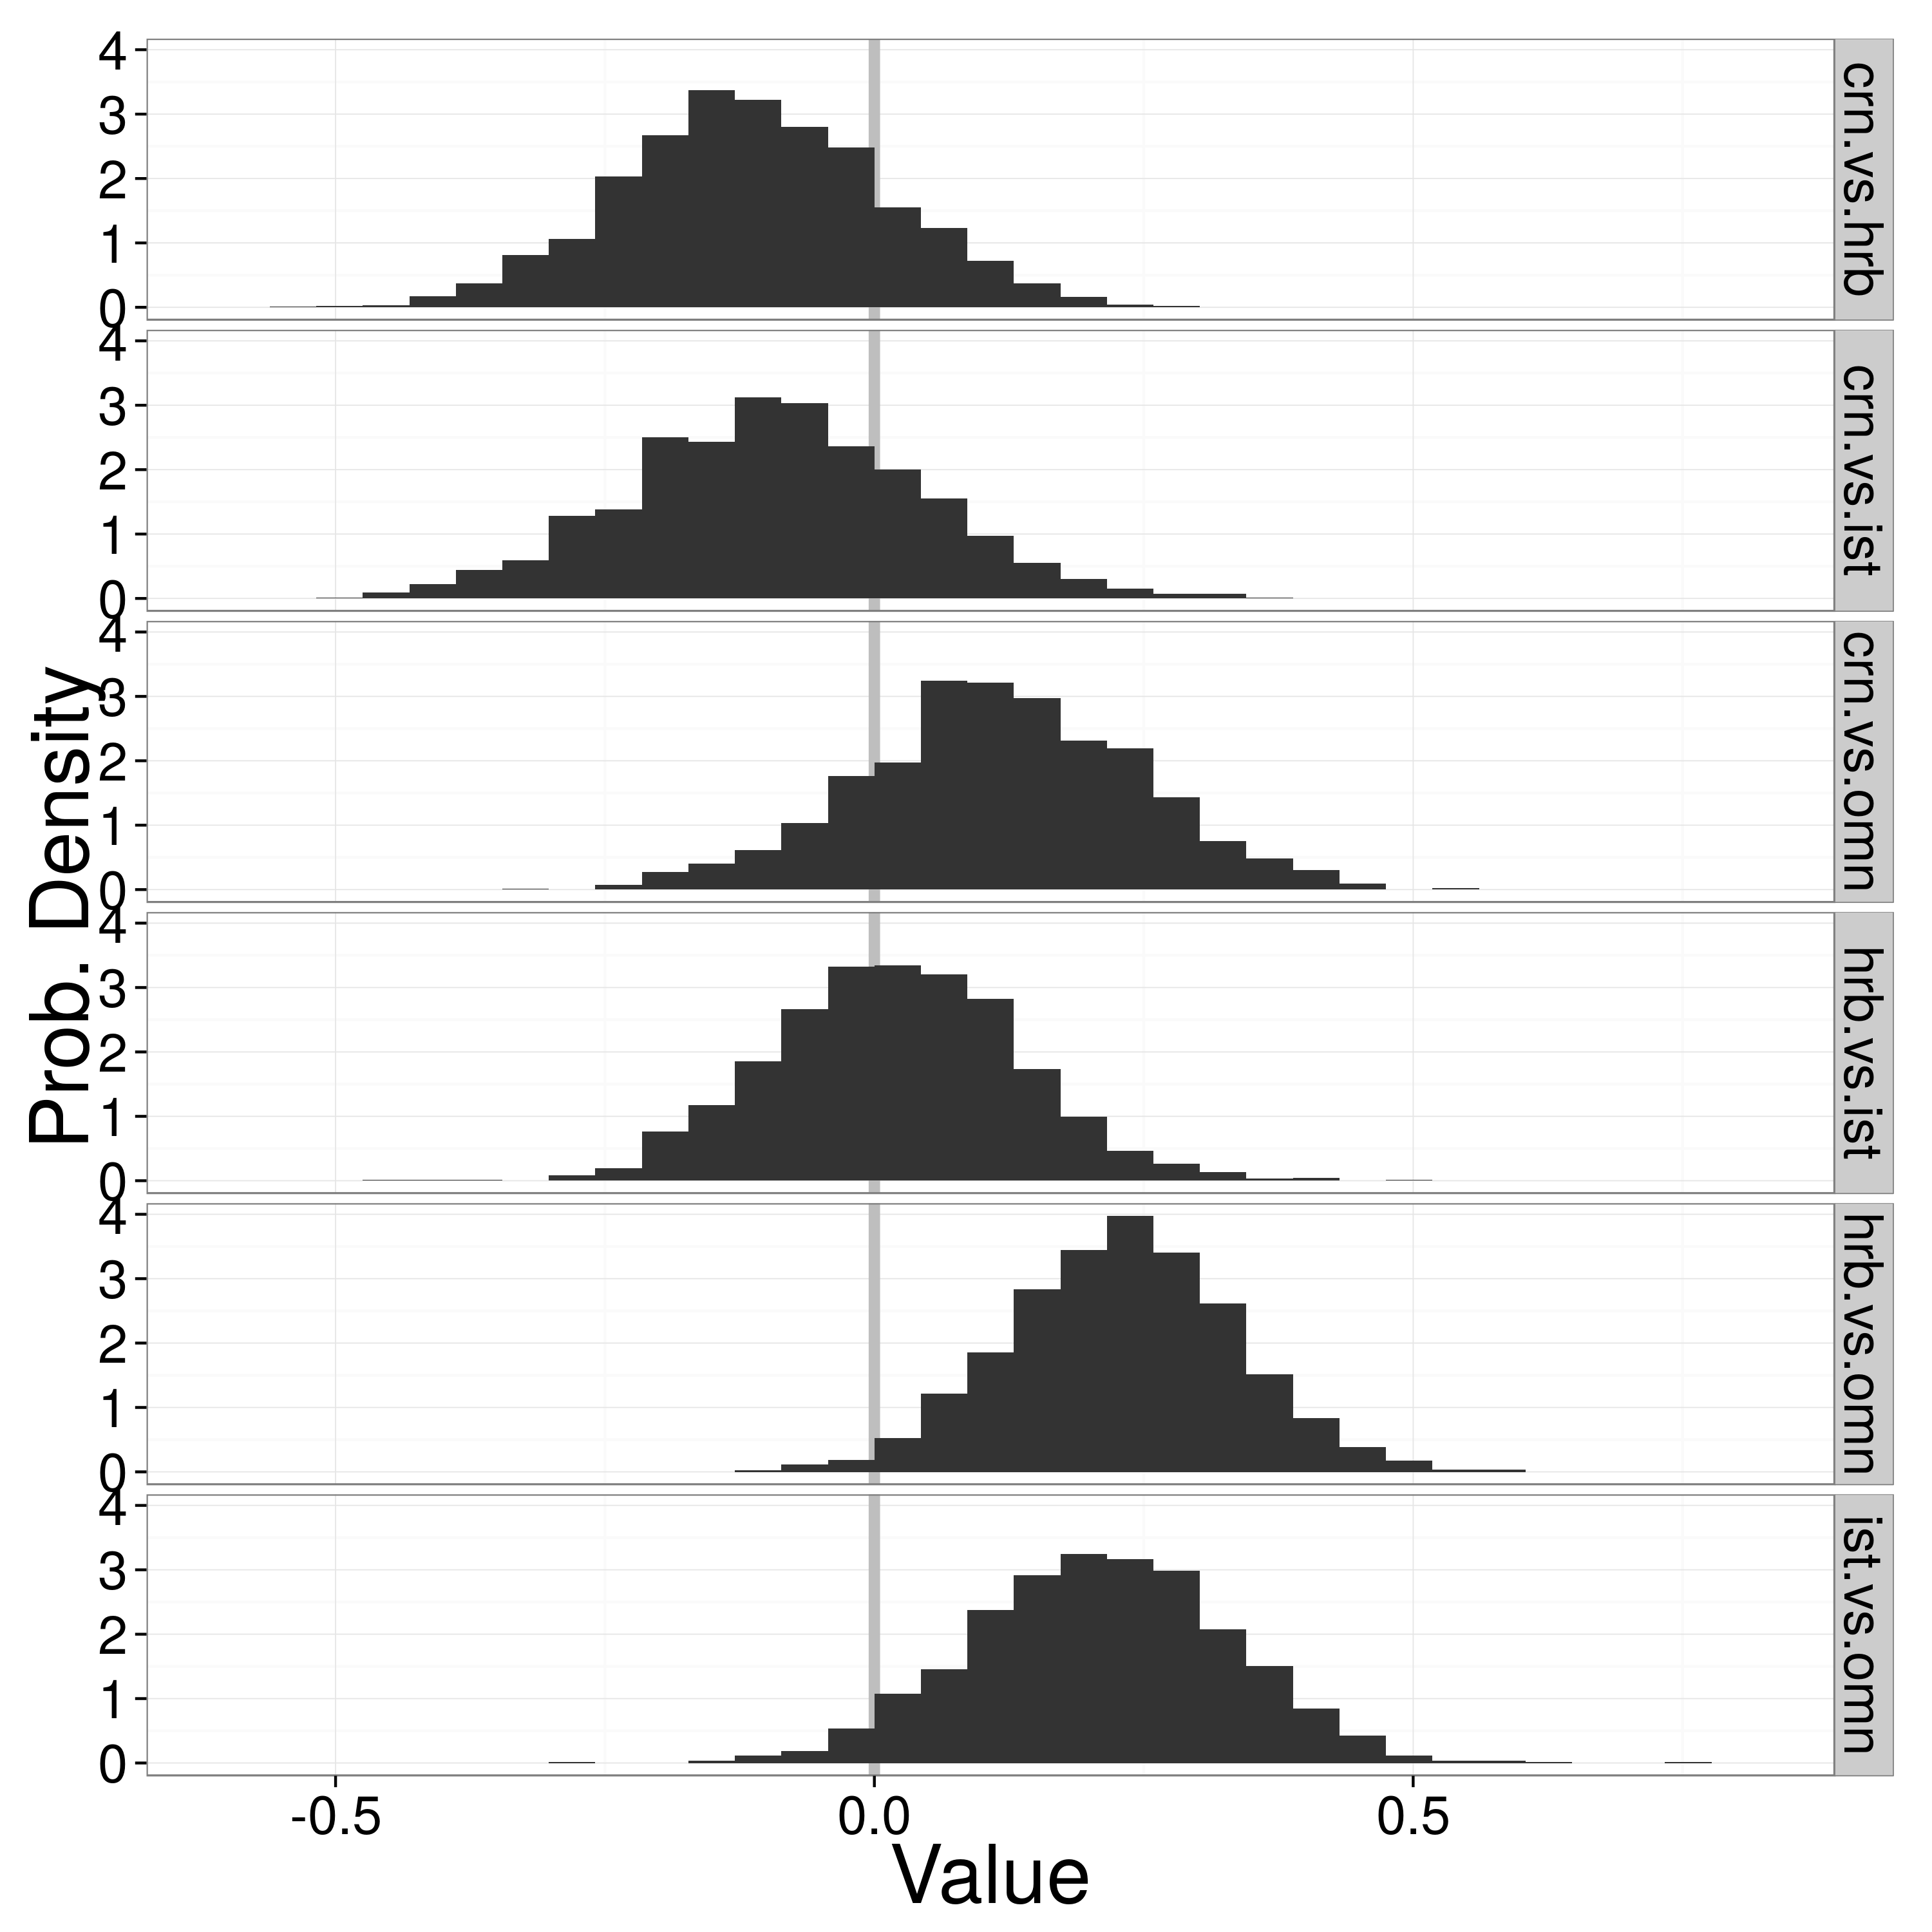
\includegraphics[height = 0.8\textheight, width = \textwidth,  keepaspectratio = true]{figure/diet_diff_est}
  \end{center}
\end{frame}

\begin{frame}
  \frametitle{Pairwise differences of \(\beta\), locomotor category}
  \begin{center}
    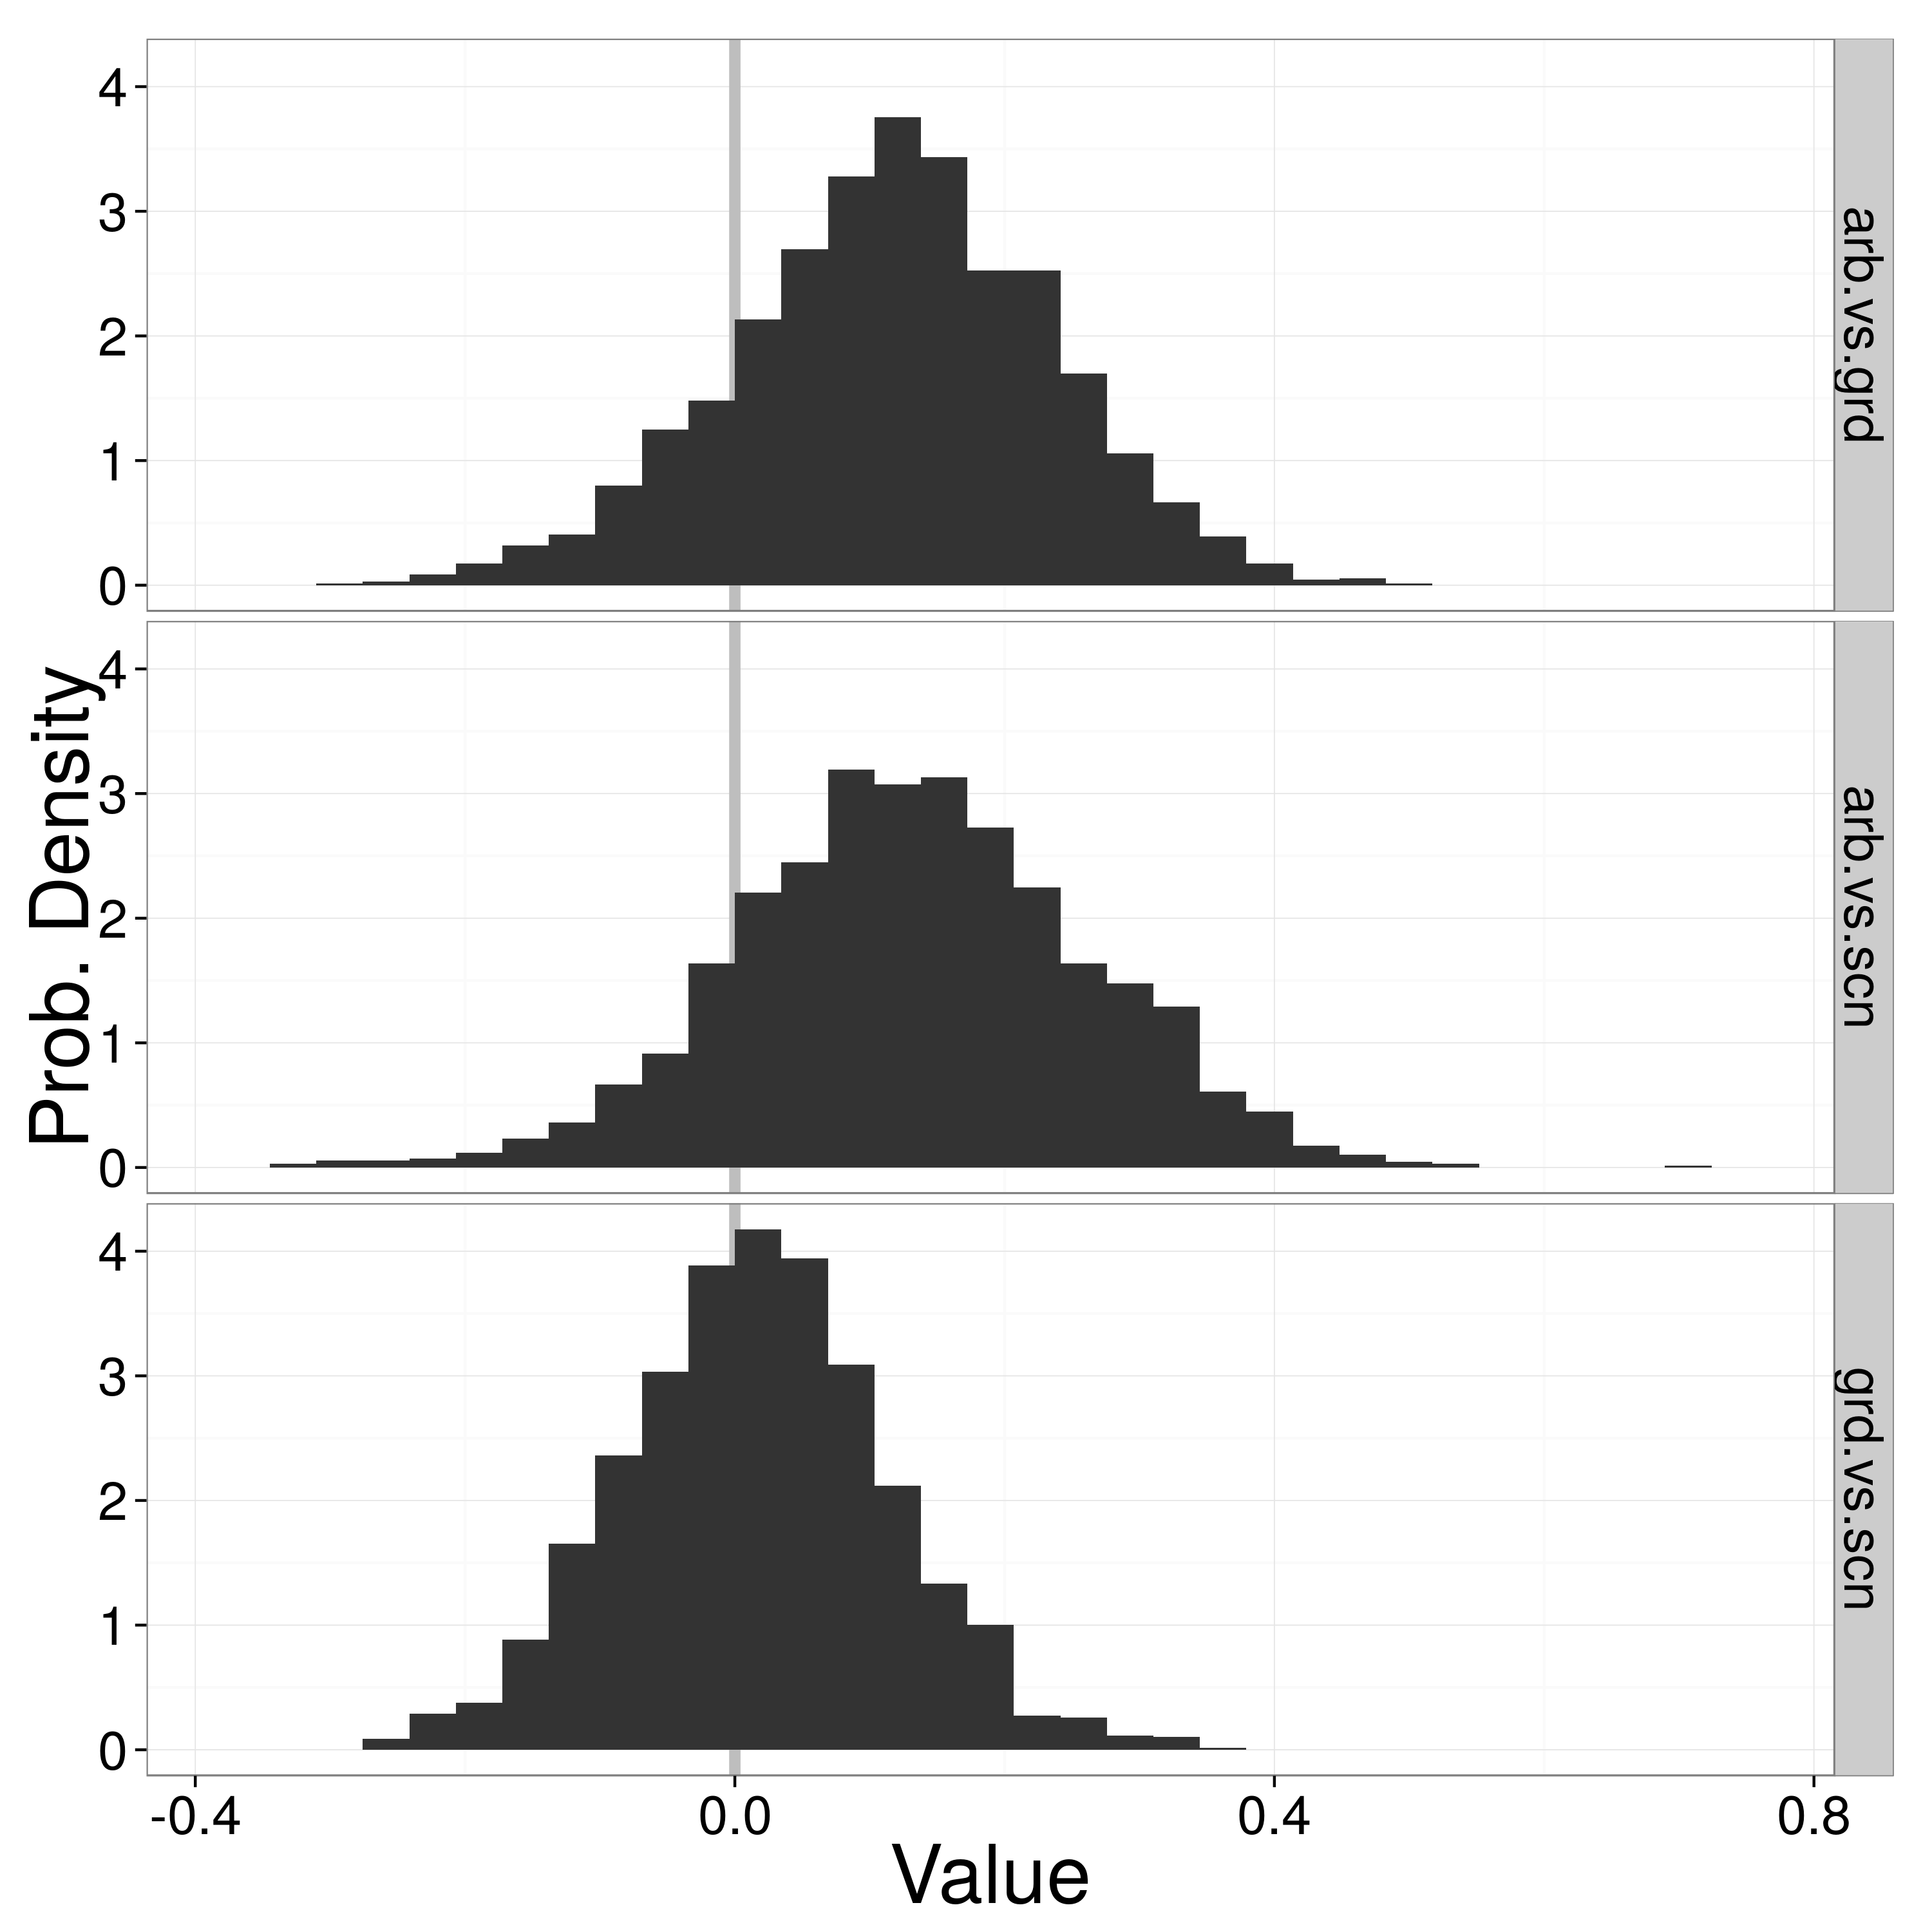
\includegraphics[height = 0.8\textheight, width = \textwidth,  keepaspectratio = true]{figure/loco_diff_est}
  \end{center}
\end{frame}

\begin{frame}
  \frametitle{Other traits}
  \begin{center}
    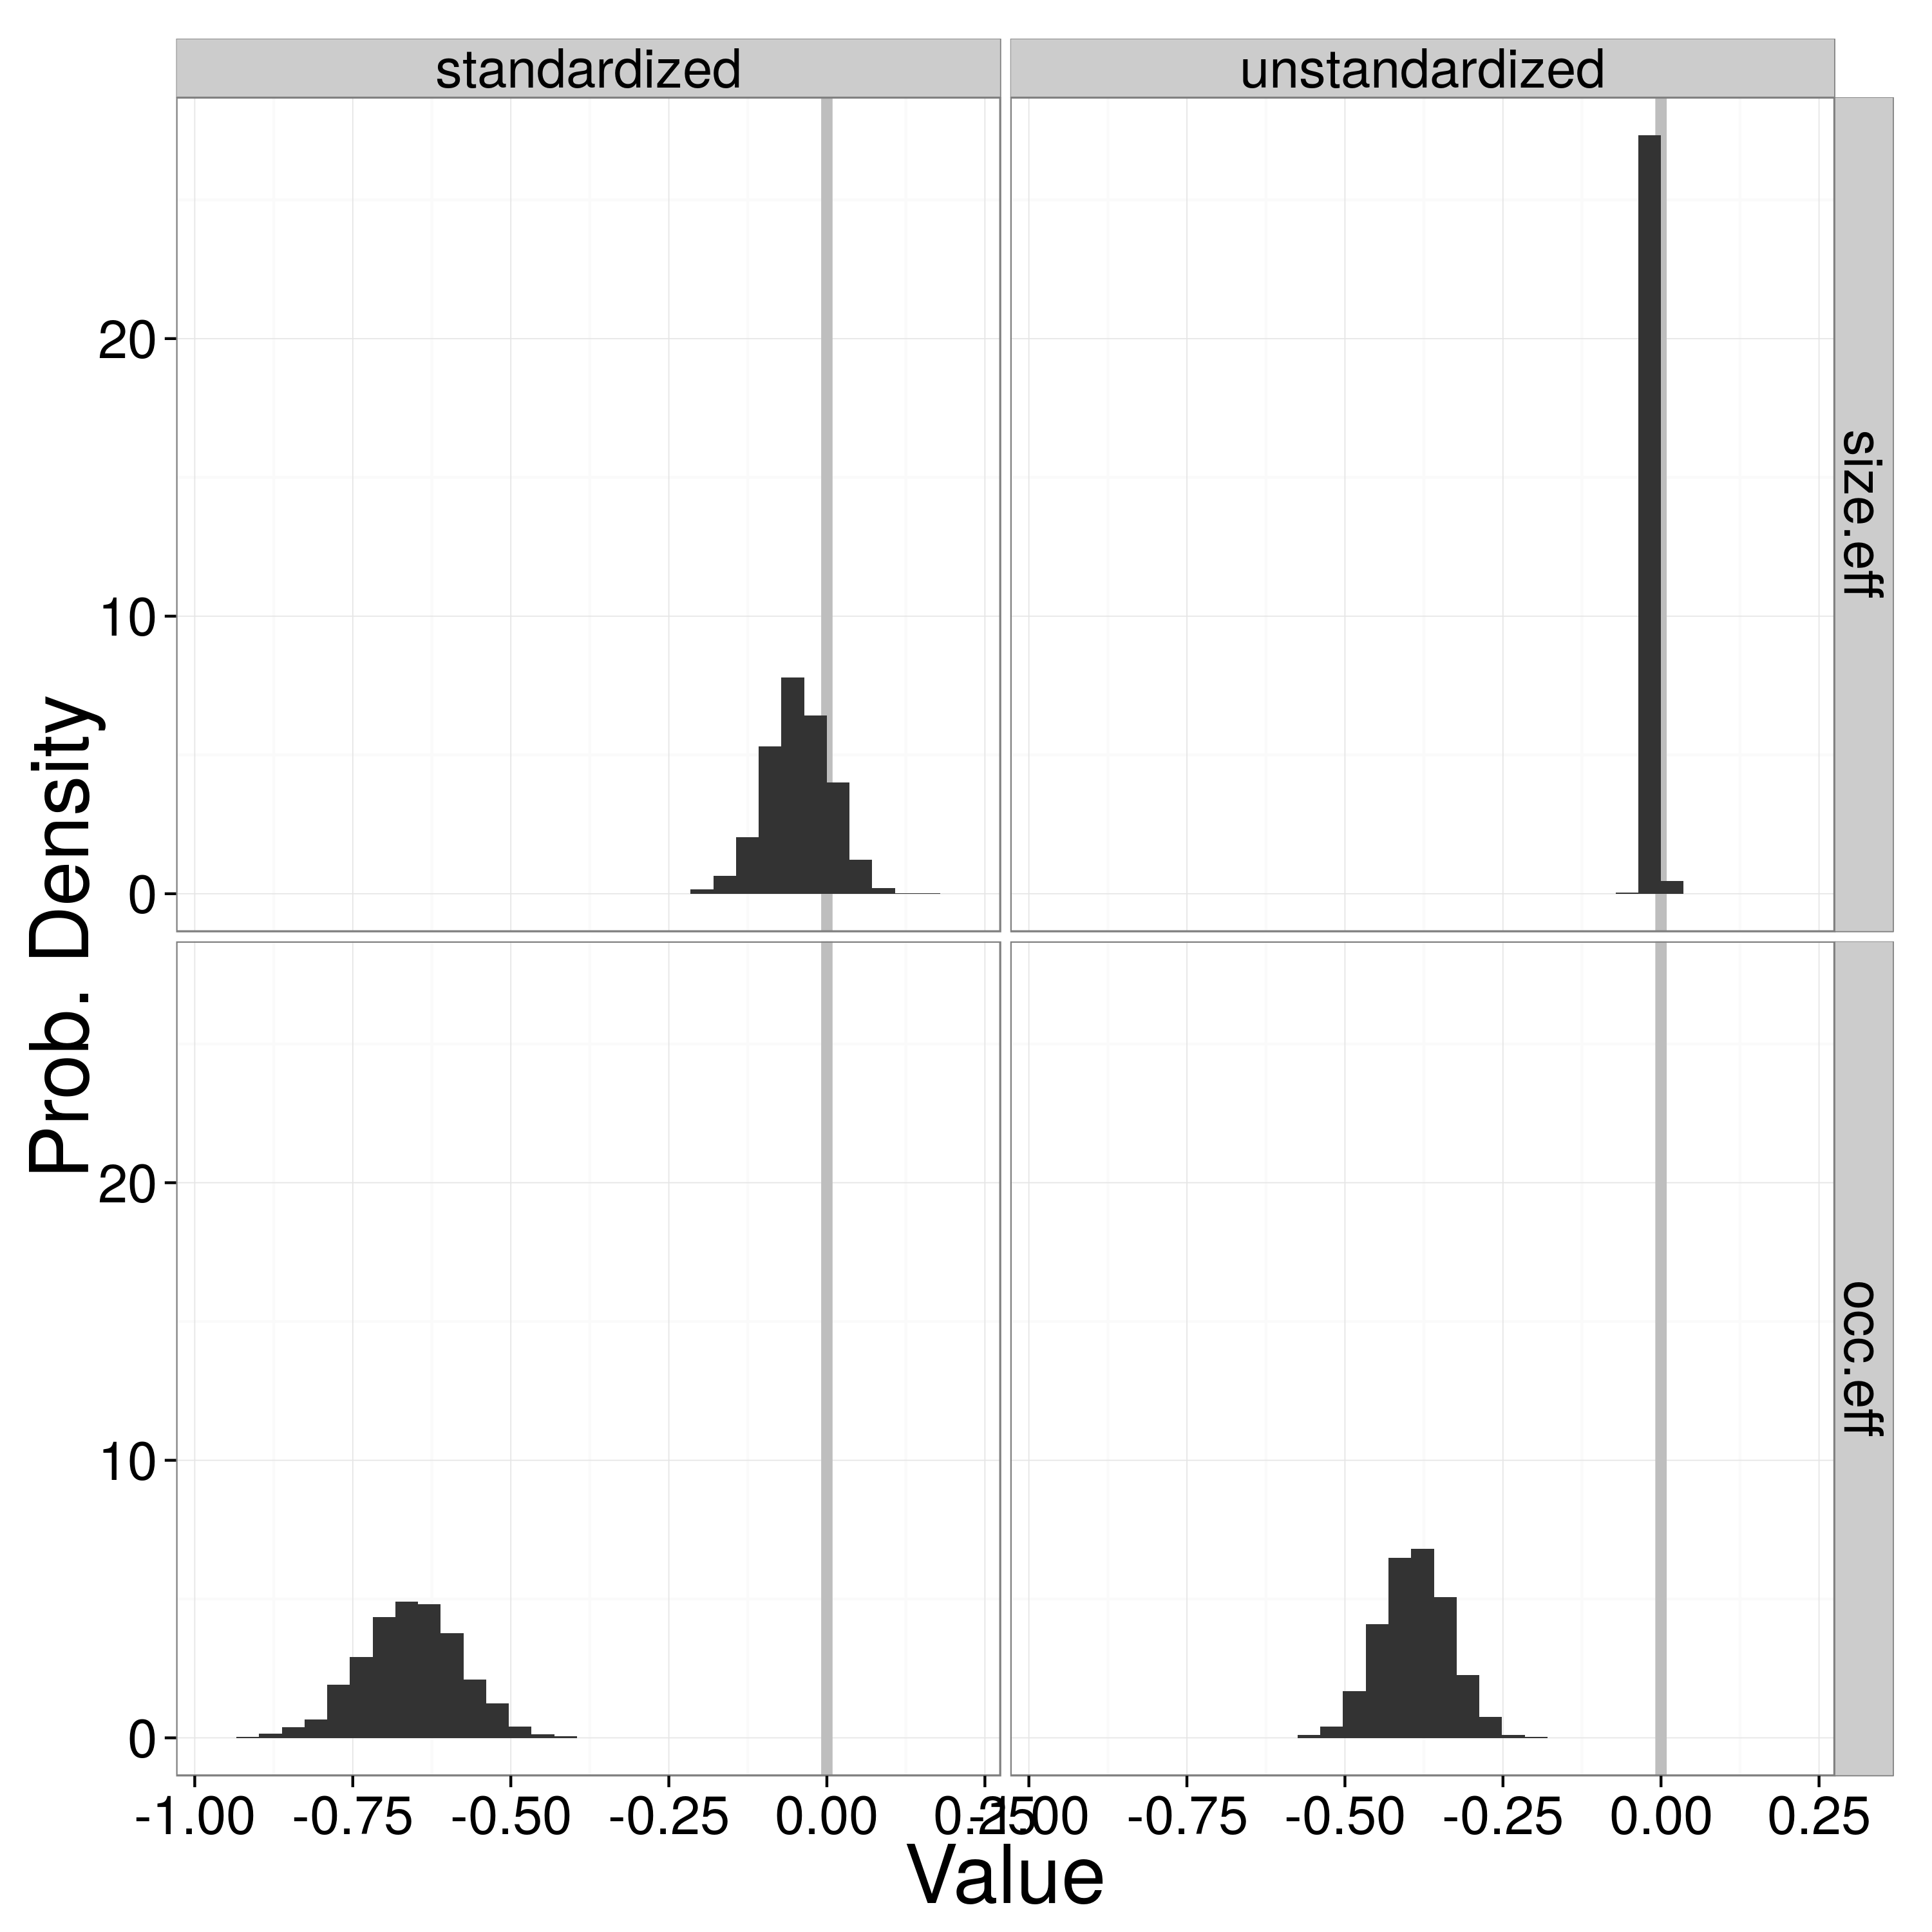
\includegraphics[height = 0.8\textheight, width = \textwidth,  keepaspectratio = true]{figure/other_est}
  \end{center}
\end{frame}

\begin{frame}
  \frametitle{Cohort effect}
  \begin{center}
    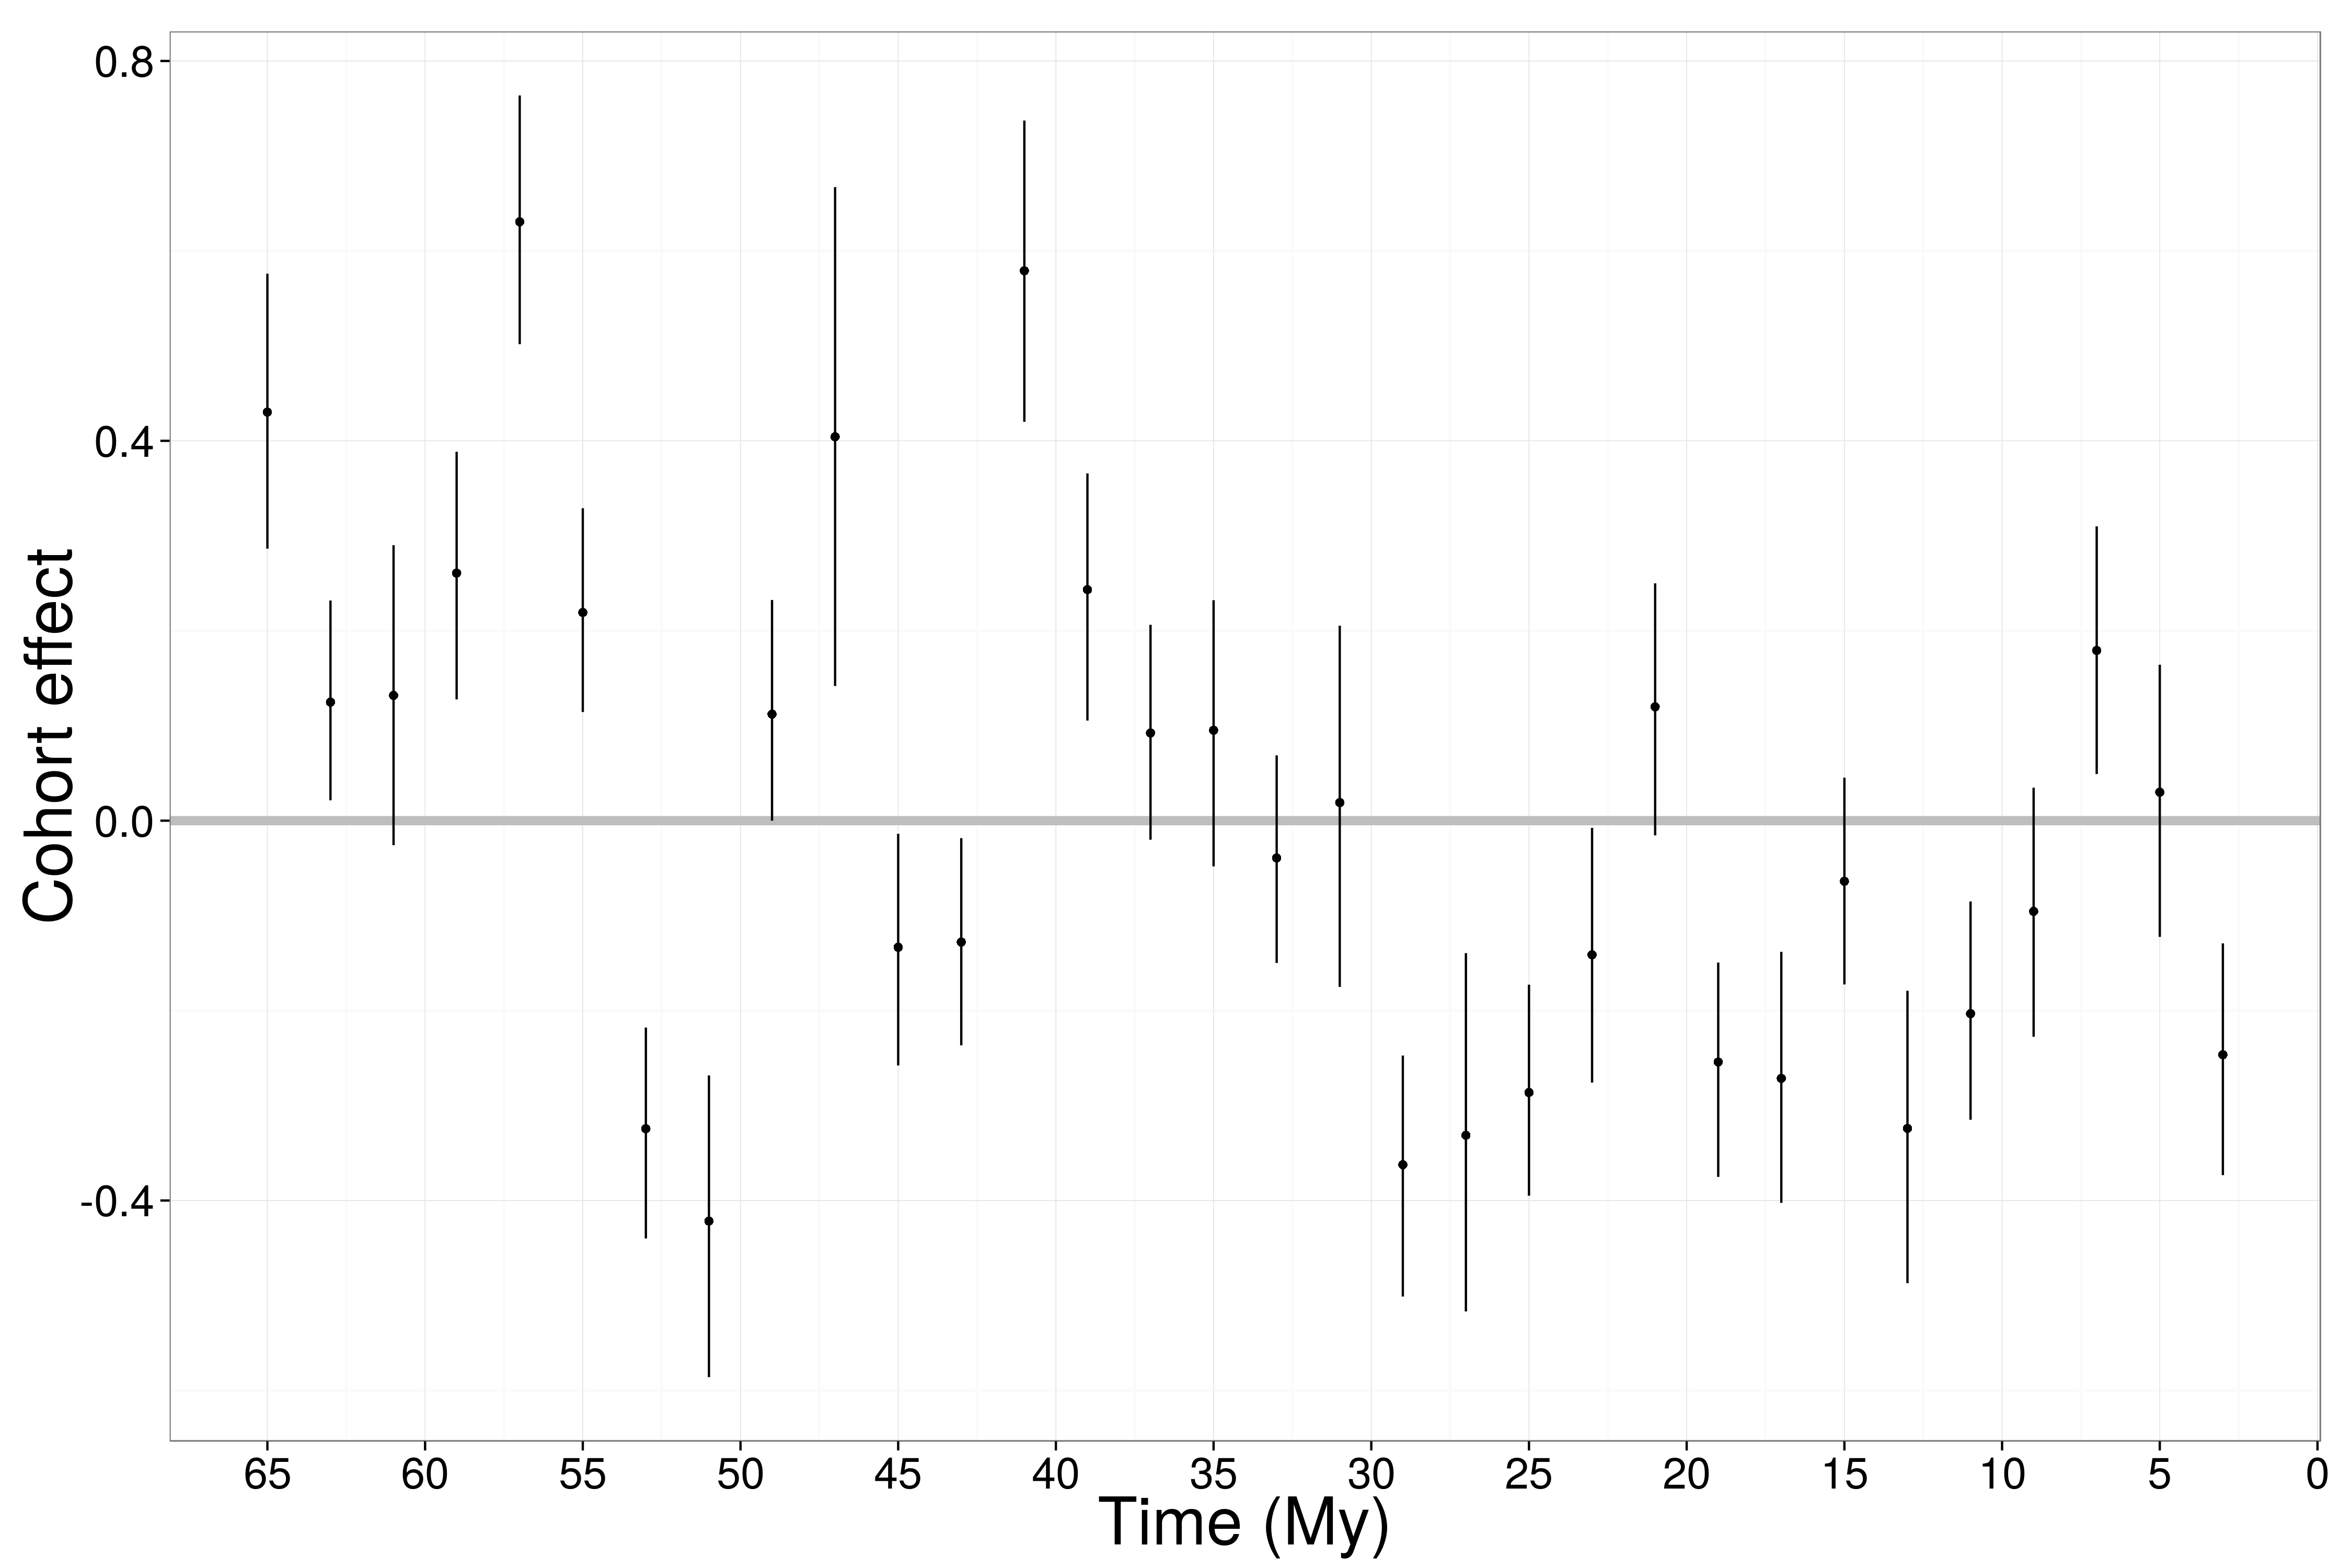
\includegraphics[height = 0.8\textheight, width = \textwidth,  keepaspectratio = true]{figure/cohort_est}
  \end{center}
\end{frame}

\begin{frame}
  \frametitle{Hazard curvature}
  \begin{center}
    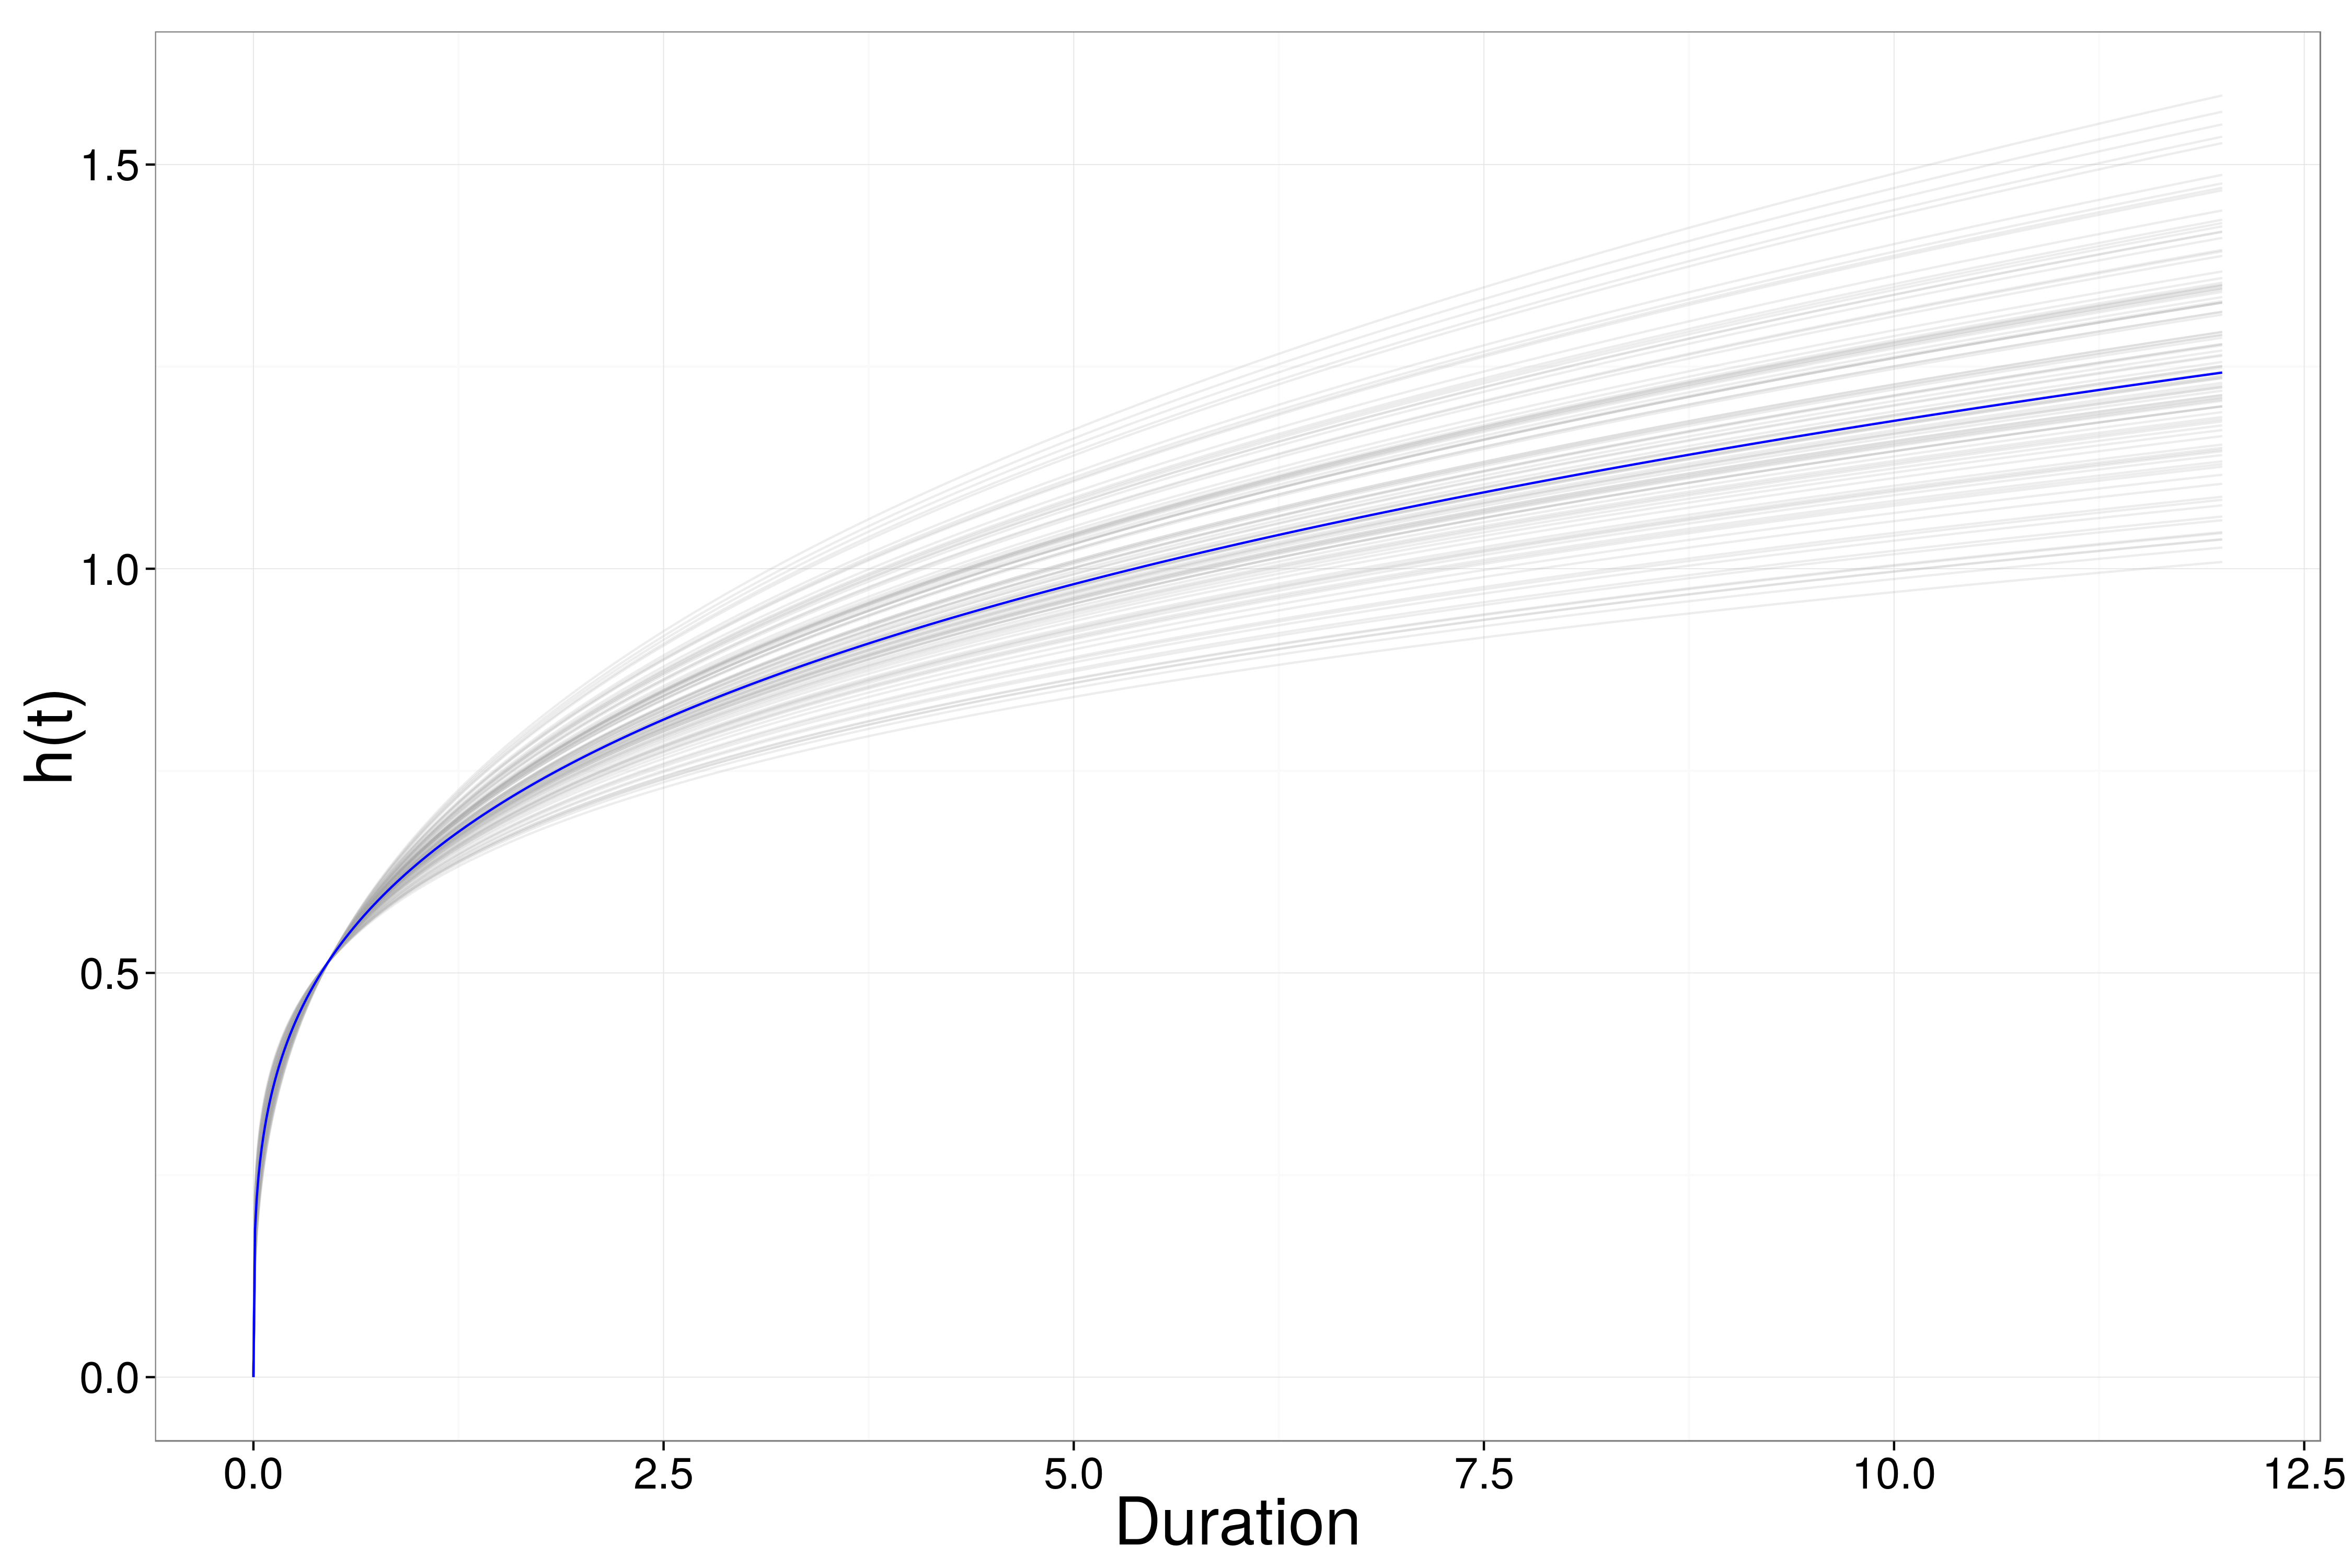
\includegraphics[height = 0.8\textheight, width = \textwidth,  keepaspectratio = true]{figure/haz_est}
  \end{center}
\end{frame}


\end{document}
